\documentclass[12pt]{book} 

\usepackage{amsmath}
\usepackage{graphicx}
\usepackage{import}
\usepackage{amsfonts}
\usepackage{booktabs}

\setlength{\parindent}{0em}  % sets auto indent at new paragraph to none

\newcommand{\incfig}[1]{%
    \import{./figures/}{#1.pdf_tex}
}

\title{\coursetitle\linebreak\lecturename}
\author{\\Cain Susko\\ 
           \\ \\ \\
      Queen's University 
    \\School of Computing\\} 

%=-=-=-=-=-title-=-=-=-=-=%
\newcommand{\lecturename}{Machine Representation of Programs: Procedures 1}
\newcommand{\coursetitle}{Computer Architecture}
%=-=-=-=-=-#####-=-=-=-=-=%

\begin{document}
\begin{titlepage}
        \maketitle
\end{titlepage}


\section*{Procedures}
a procedure is a list of instructions that allow a computer/CPU to do various complex tasks. They are also known as 
        functions which alludes to their manifestation; code!

\begin{figure}[h]
        \centering
        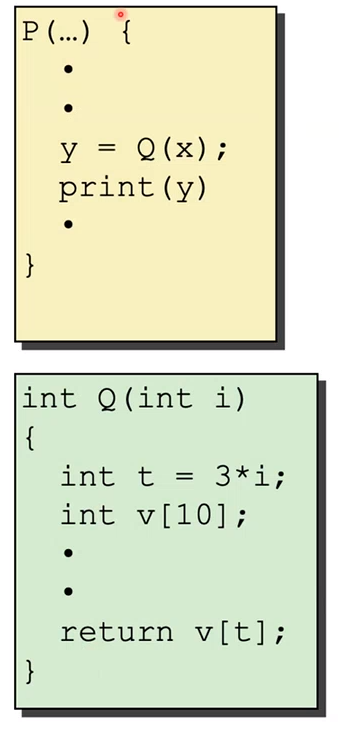
\includegraphics[scale = 0.5]{./figures/procedureEx}
        
\end{figure}

There can be many procedures that a computer can run, thus there is also a passing of control between procedures. This 
passing of control also tends to pass data (ie. Input parameter, return variable) 
\pagebreak


\section*{Stack Structure}
The stack structure is dependent on the architecture and operating system being used. The x84-64 stack is defined as:
\begin{figure}[h]
        \centering
        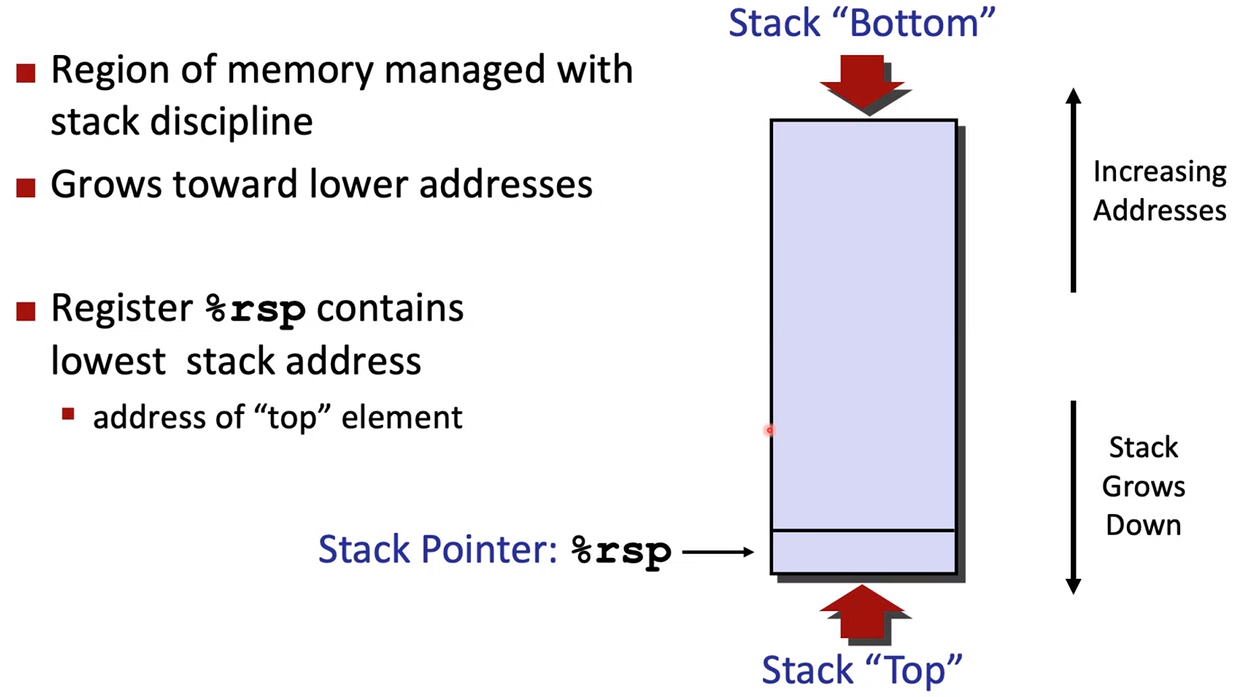
\includegraphics[scale = 0.4]{./figures/x86stack}
\end{figure}

With the stack we can read and write to it using pust and pop:
\begin{itemize}
        \item[\texttt{pushq Src}] Fetch operand at \texttt{Src}. Decrement \texttt{\%rsp} by 8. Write operand to 
                address given by \texttt{\%rsp}
        \item[\texttt{popq dest}] Read value at address given by \texttt{\%rsp}, 
                incrament \texttt{\%rsp} by 8 (because we are using a 64 bit architecture) and store the value at
                \texttt{dest} (Note: $dest$ must be a register)
\end{itemize}

Whithin the context of procedures, the stack within the architecture allows for passing of control between procedures.
For example:
\begin{figure}[h]
        \centering
        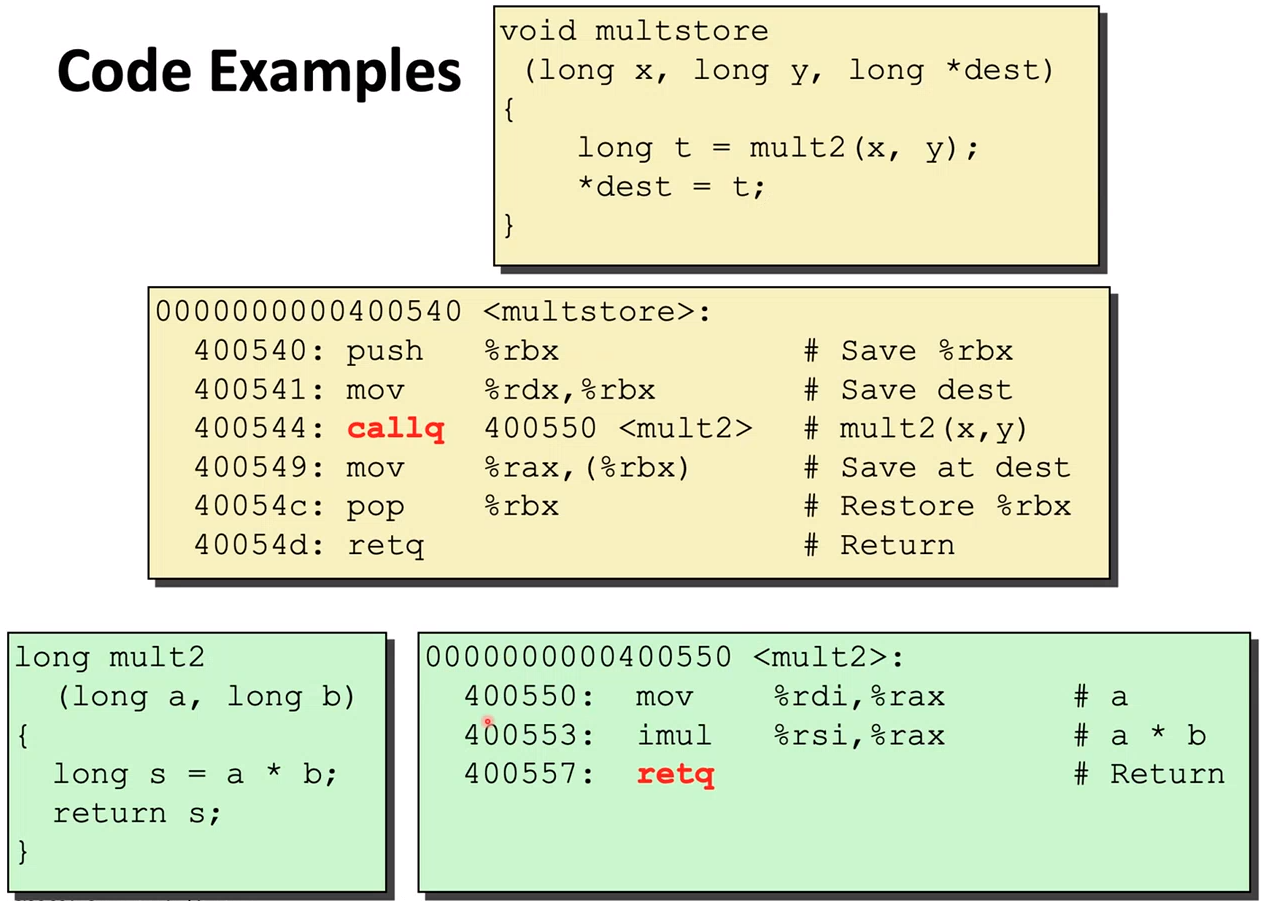
\includegraphics[scale = 0.1]{./figures/procedureCode}
\end{figure}

\section*{Procedure Control Flow}
We use the stack to support procedure $call$ and  $return$.
\begin{itemize}
        \item[\texttt{call label}] pushes return address onto stack and jumps to label.
        \begin{itemize}
                \item Return Address: address of next instruction right after call.
        \end{itemize}
        \item[\texttt{ret}] pop (returns) address from stack and jumps to address.
\end{itemize}

Below is an example of a stack control flow in x86-64 architecture:
\begin{figure}[h]
        \centering
        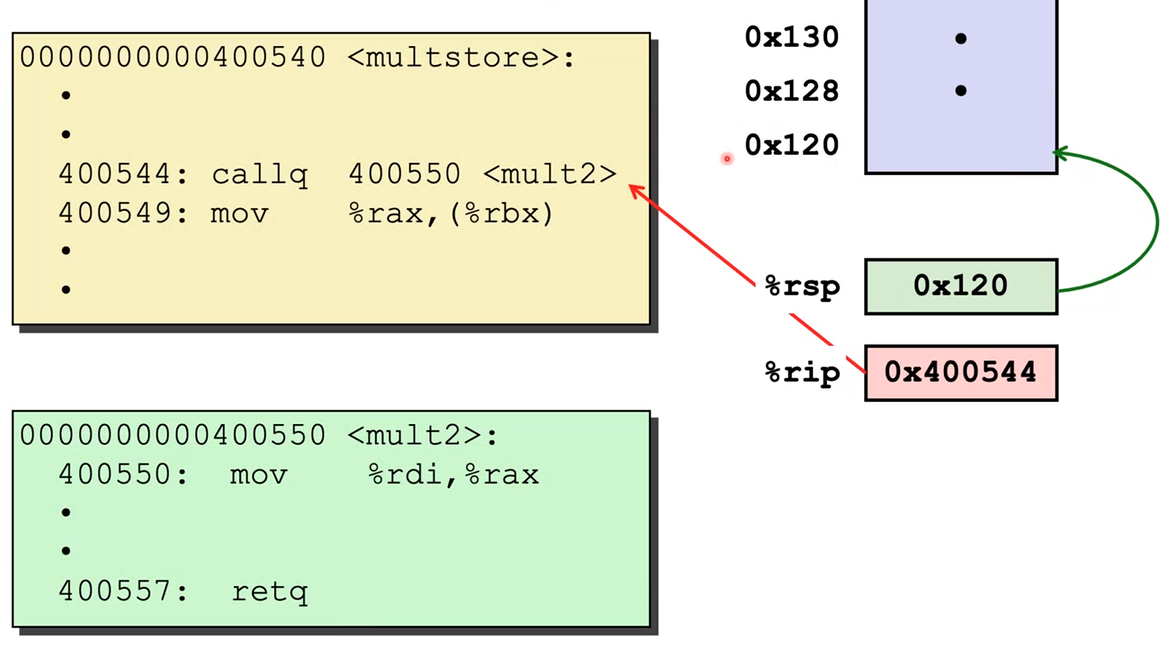
\includegraphics[scale = 0.3]{./figures/controlflowEx}
\end{figure}
\begin{itemize}
        \item first, our pointer on the stack $\%rsp$ and the program counter  $\%rip$. The next step is to move to 
                a new procedure.
        \item $\%rip$ is now pointing to the first part of the green procedure and  $\%rsp$ pushed the address
                of the previous place onto the stack
        \item as  $\%rip$ moves along the new function it reaches the return call, where it then gets the value from the
                stack by popping the top of the stack into the program counter.
\end{itemize}
\pagebreak


\section*{Procedure Data Flow}
Data flow is achieved by using registers for the first 6 arguments of a procedure
and 1 for the return value. The stack holds all remaining 
arguments.

An example of Data Flow with less than or equal to 6 arguments:
\begin{figure}[h]
        \centering
        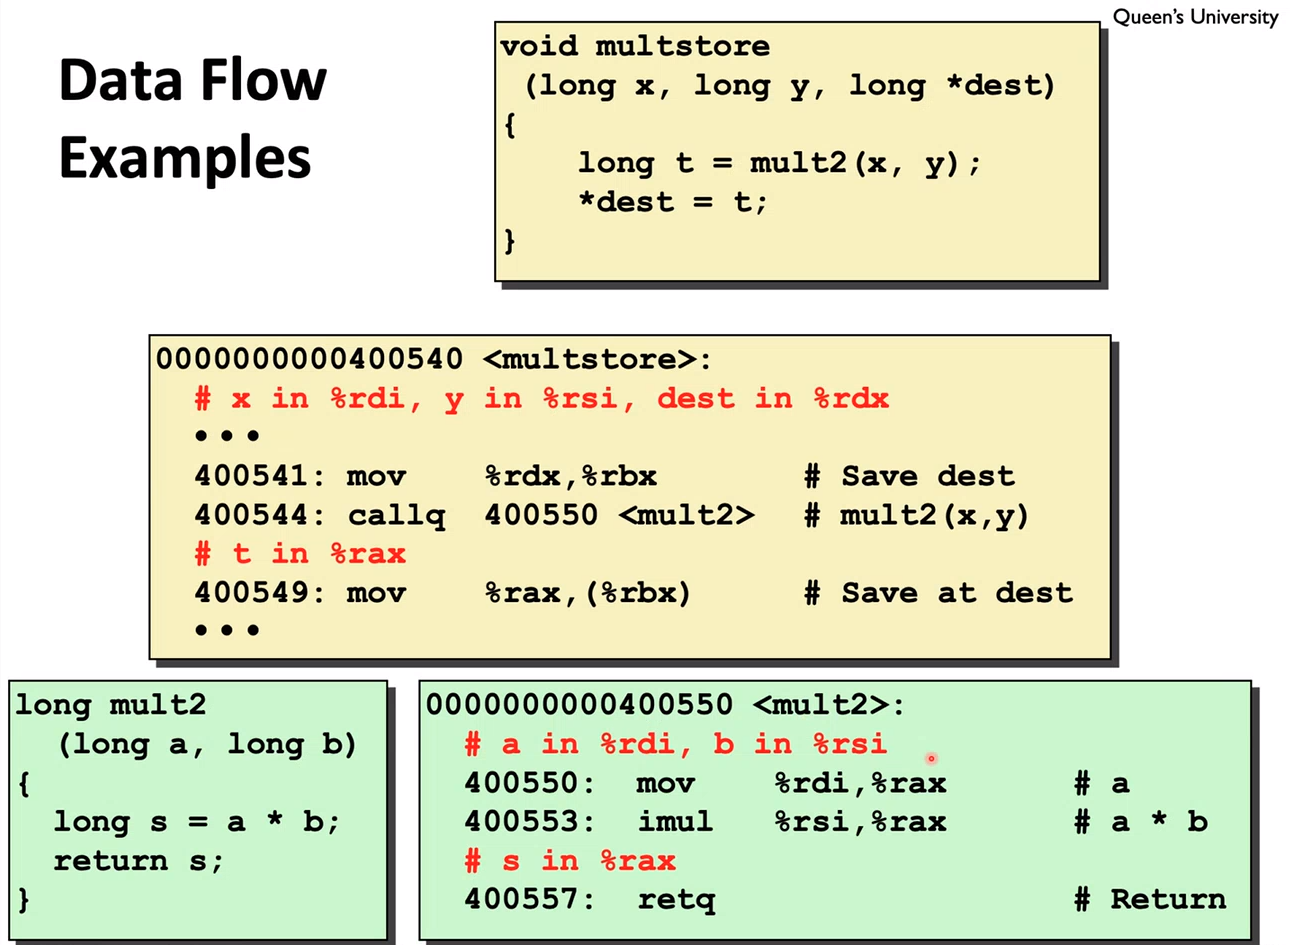
\includegraphics[scale = 0.2]{./figures/dataflowEx}
\end{figure}

\section*{Managing Local Data}
Most modern Languages support recursion or are `reentrant'. 
Becuase of this, the languages need a place to store the multiple concurrent instances of a procedure.

\begin{figure}[h]
        \centering
        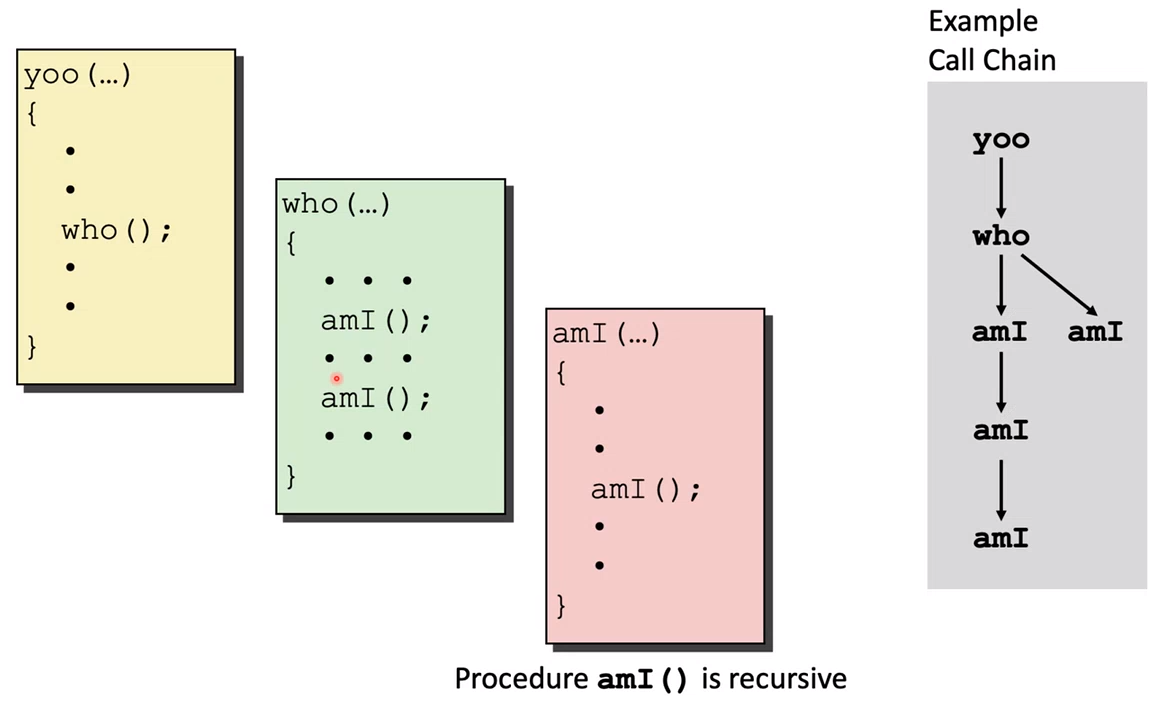
\includegraphics[scale = 0.2]{./figures/callchain}
\end{figure}

Within the stack, the state for a given procedure is needed only for a limited time: from when it is called
to when it is returned. Additionally, the callee returns before the caller does. These are a part of whats known as 
stack discipline.

Finally, the stack is allocated in $frames$ where each frame is a state for a single procedure
instantiation.

\paragraph{Stack Frame}
Each stack frame contains space that we need for temporary storage for local variables.
\begin{itemize}
        \item return information
        \item local storage
        \item temporary space
\end{itemize}

The computer must also manage these frames (obviously).
\begin{itemize}
        \item space is allocated when entering a procedure. Manifests as setup code with a push by \texttt{call}
                instruction
        \item space is deallocated on return. Manifests as finishing code which includes a pop by \texttt{ret}
                instruction
\end{itemize}

With reference to the previous representation of the stack, frames are stored using an (optional) frame pointer: 
commonly, \texttt{\%rbp}.

\begin{figure}[h]
        \centering
        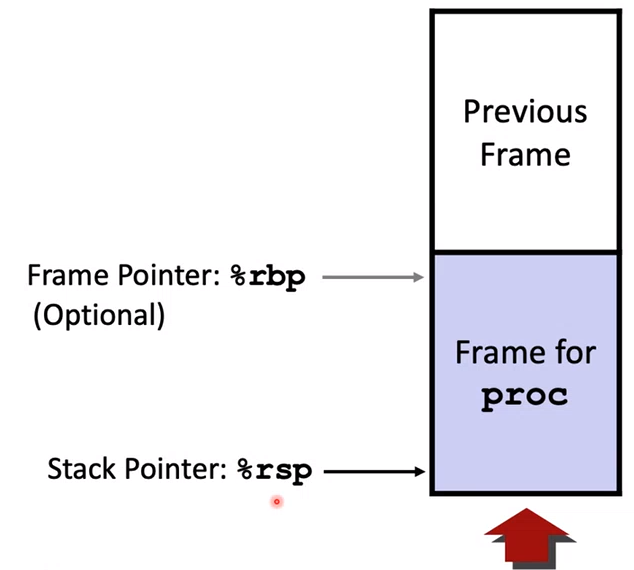
\includegraphics[scale = 0.4]{./figures/stackframe}
\end{figure}

Note: all variables for \texttt{proc} are within the frame, between \texttt{\%rbp \& \%rsp}
\pagebreak

For many functions being called or cany instances of the same function being called, the stack and it's frames
would look like so:
\begin{figure}[h]
        \centering
        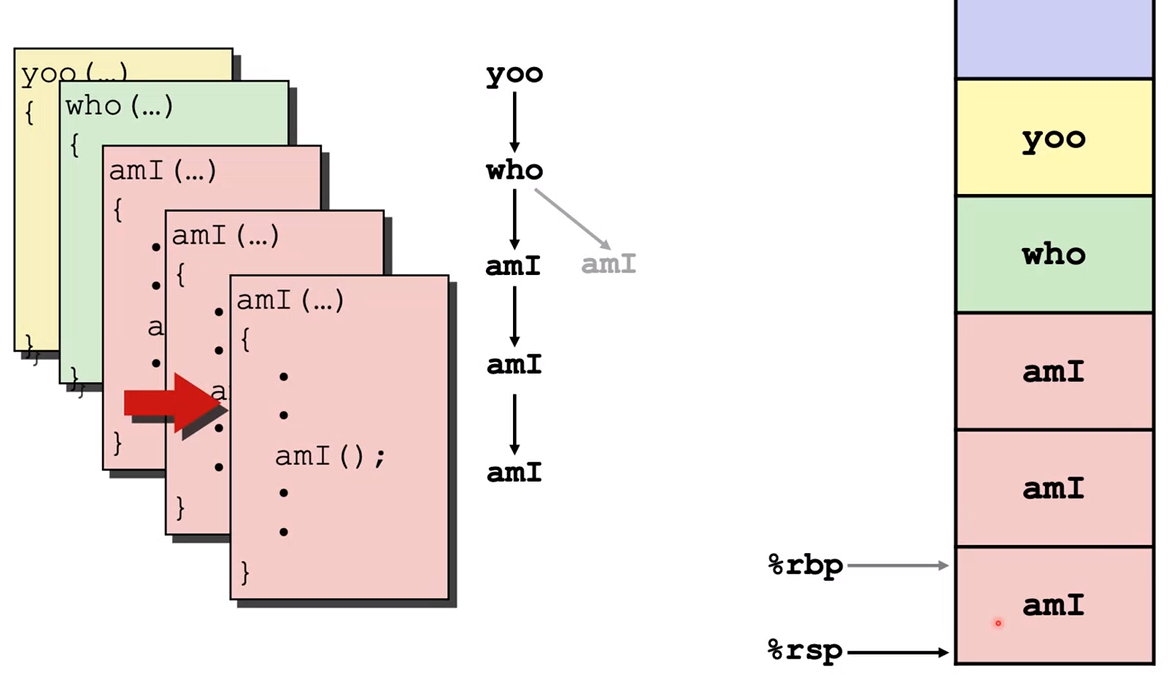
\includegraphics[scale = 0.3]{./figures/stackframeMany}
\end{figure}

\paragraph{x86 Linux} 
Within the x86-64 architecture on a linux system, a stack is structured like so:
\begin{figure}[h]
        \centering
        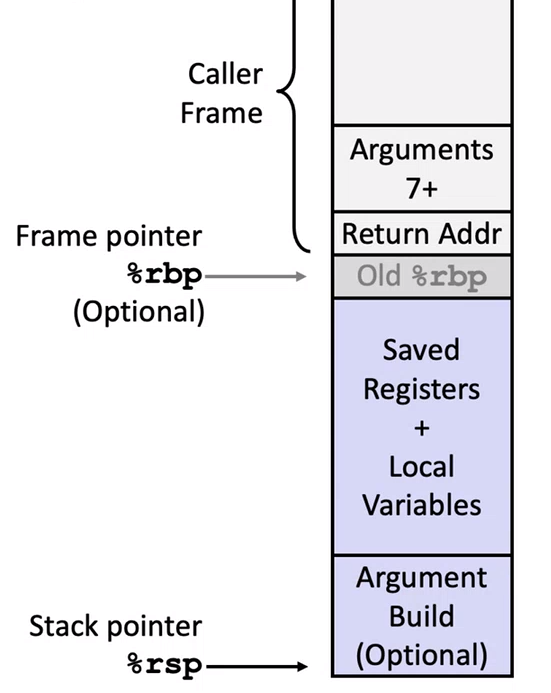
\includegraphics[scale = 0.3]{./figures/x86stackframe}
\end{figure}

Where:
\begin{itemize}
        \item the current stack frame contains:
                \begin{itemize}
                        \item Argument Build - parameters for function that is about to be called.
                        \item Local Varibles - if unable to keep in registers
                        \item Saved Register Context
                        \item Old Frame Pointer - optional
                \end{itemize}
        \item the caller stack frame contains:
                \begin{itemize}
                        \item Return Address - pushed by \texttt{call} instruction.
                        \item Arguments for this Call
                \end{itemize}
\end{itemize}

An example of this local data management is that of the \texttt{incr} function, which incraments a variable.
\begin{figure}[h]
        \centering
        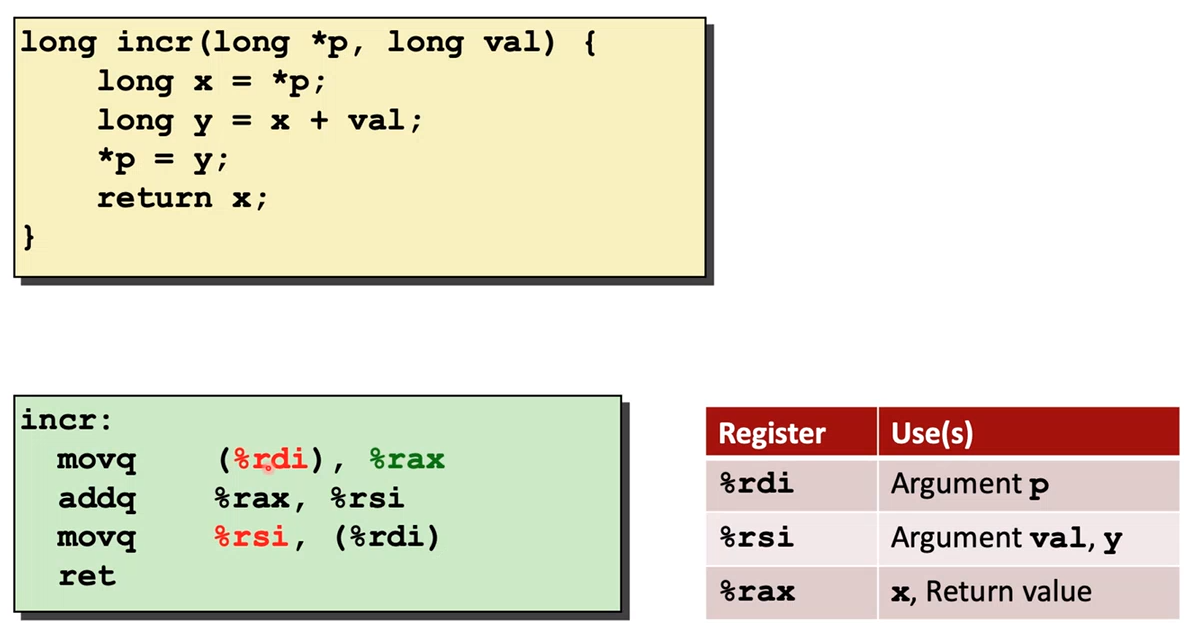
\includegraphics[scale = 0.2]{./figures/localdataEx}
        
\end{figure}

The implementation of this function is:
\begin{figure}[h]
        \centering
        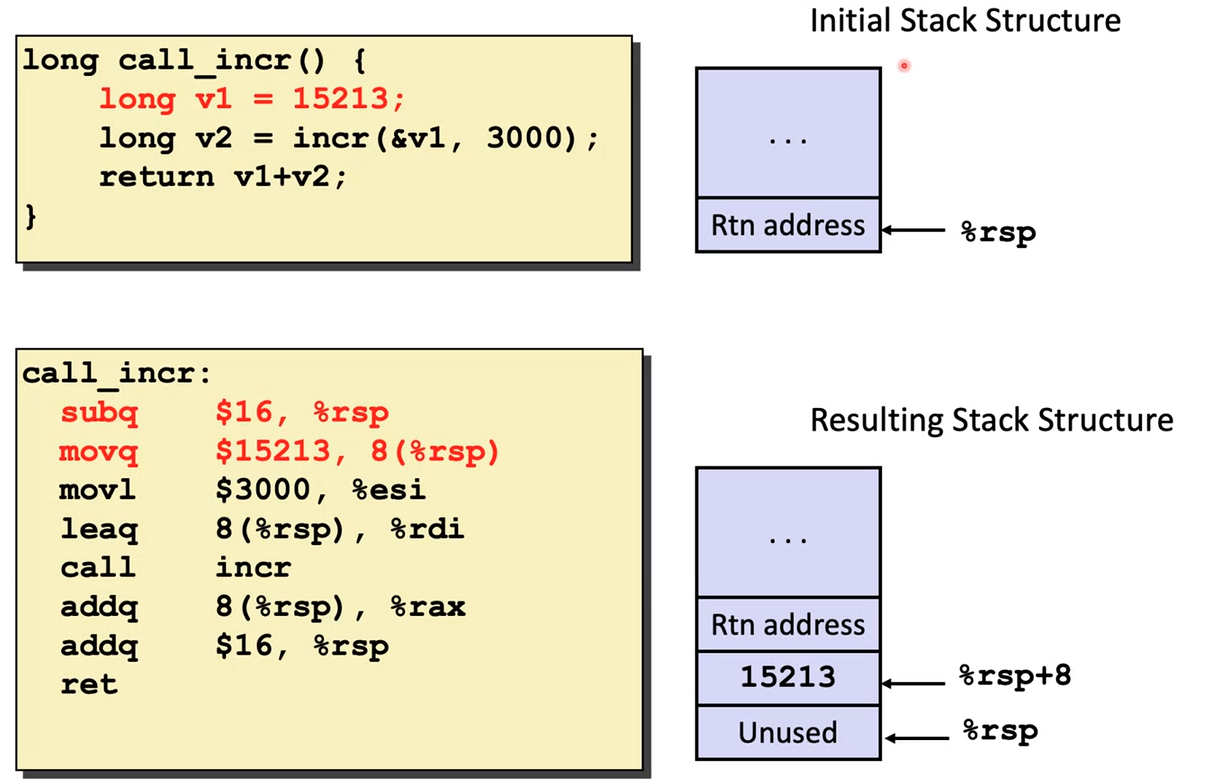
\includegraphics[scale = 0.2]{./figures/localdataEx2}
\end{figure}

And as the program progresses, the stack and it's frames are updated as needed.

\begin{figure}[h]
        \centering
        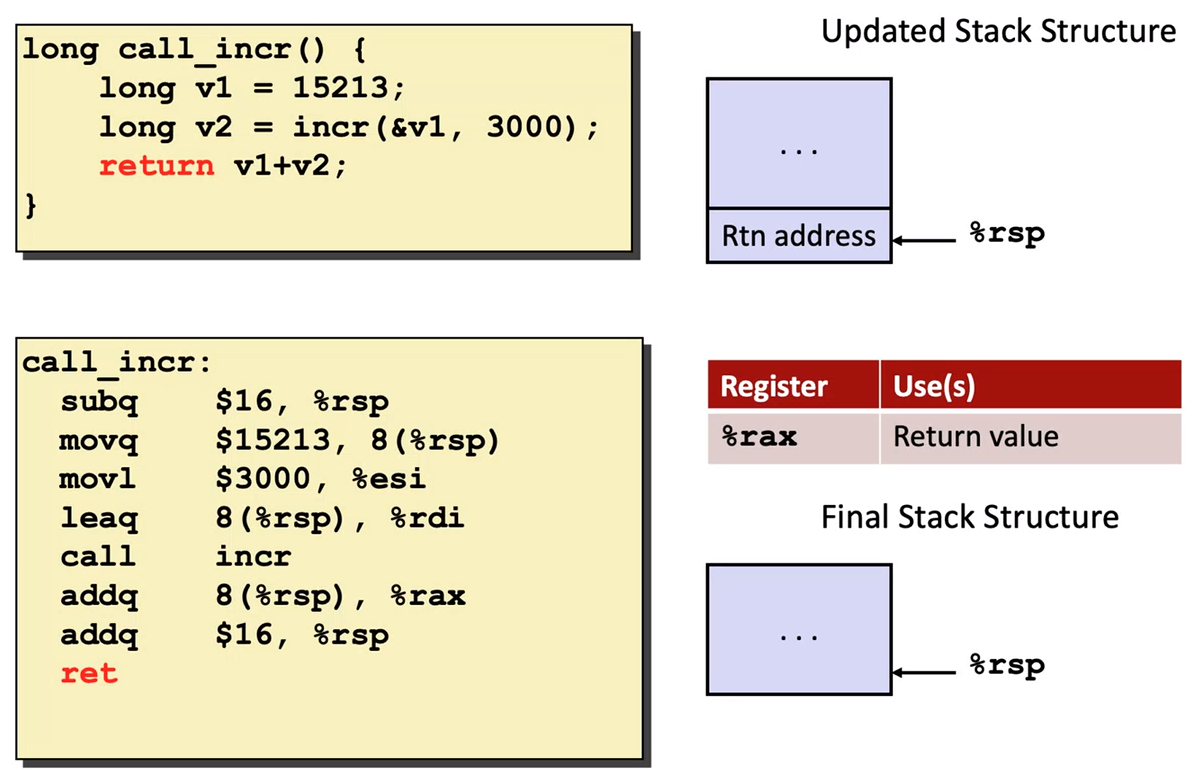
\includegraphics[scale = 0.17]{./figures/localdataEx3}        
\end{figure}
\end{document}

